\chapter{サンプル}
\label{chap:ch01}

\begin{quotation}
書き方のサンプルです。上書きするなりして消して下さい。
\end{quotation}

\section{本文の書き方}
\label{sec:1-1}

最初の段落です。
この行も同じ段落です。

次の段落です。

2行以上以上空いていても1行空いているのと同様に処理します。

\subsection{見出し}
\label{sec:1-1-1}

「=」「==」「===」の後に一文字空白をあけると見出しになります。

\begin{reviewcolumn}
\hypertarget{column:ch01:1}{}
\reviewcolumnhead{}{コラムについて}

見出しの先頭に「[column]」と書くと、そこはコラムになります。

\end{reviewcolumn}

\section{箇条書き}
\label{sec:1-2}

番号のない箇条書きは「*」を使います。前後に空白を入れて下さい。

\begin{itemize}
\item 1つ目
\item 2つ目
\item 3つ目
\end{itemize}

番号つきの箇条書きには、「1.」「2.」などと書きます。
数字の値は実際には無視され、連番が振られます。

\begin{enumerate}
\item 1つ目
\item 2つ目
\item 3つ目
\end{enumerate}

\section{ソースコードなどのリスト}
\label{sec:1-3}

リストには「//list」ブロックや「//emlist」ブロックを使います。

\reviewlistcaption{リスト1.1: リストのサンプル}
\begin{reviewlist}
int main(int argc, char **argv) \{
  puts("OK");
  return 0;
\}
\end{reviewlist}

文中にリストを書くには「//emlist」になります。

\begin{reviewemlist}
def main
  puts "ok"
end
\end{reviewemlist}

\section{画像}
\label{sec:1-4}

画像は「//image」ブロックを使います。

\begin{reviewimage}
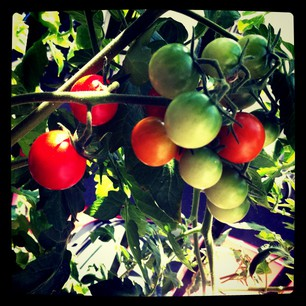
\includegraphics[width=\maxwidth]{./images/ch01-imgsample.jpg}
\caption{画像サンプル}
\label{image:ch01:imgsample}
\end{reviewimage}

より詳しくは、
\url{https://github.com/kmuto/review/blob/master/doc/format.rdoc}
を御覧ください。
